\chapter{Optimización de consultas}

Organizar más adecuadamente la información a nivel físico no es lo único por hacer cuando se optimiza el funcionamiento de una BD. Las operaciones más ejecutadas en una base de datos son las consultas, y estas pueden ser optimizadas (transformadas antes de su ejecución para que se ejecuten de la forma más eficiente posible -en tiempo y espacio-), pero este proceso también gasta tiempo.

El \textbf{optimizador} es el módulo del SGBD que efectúa modificaciones en la consulta para obtener los datos consultados de la forma más eficiente tratando de reducir:
\begin{enumerate}[(a)]
\item El tiempo de evaluación o
\item El tiempo de respuesta
\end{enumerate}
El coste minimizable se base en dos costes diferentes:
\begin{enumerate}[(a)]
\item Coste de acceso a almacenamiento secundario
\item Coste computacional (basado en el número de comparaciones)
\end{enumerate}
\medskip
\begin{example}
Supongamos que tengamos la siguiente tabla en la base de datos:
\begin{itemize}
\item Alumno (DNI, nombre, fec\_nac, ciudad, direccion, tlfno, beca)
\item Asignatura (codigo, nombre, creditos, caracter, curso)
\item Matricula (codigo, DNI, calificacion)
\end{itemize}

Consulta que queremos optimizar:
\begin{lstlisting}[ language=SQL,
                    deletekeywords={IDENTITY},
                    deletekeywords={[2]INT},
                    morekeywords={clustered},
                    framesep=8pt,
                    xleftmargin=40pt,
                    framexleftmargin=40pt,
                    frame=tb,
                    framerule=0pt ]
  SELECT alumno.nombre FROM alumno, matricula 
  WHERE alumno.DNI = matricula.DNI 
  AND beca = "N" 
  AND calificacion LIKE "SOBRESALIENTE HONOR";
\end{lstlisting}

Suponiendo que la eficiencia de la ordenación es $O(n\log_2(n))$y la tabla cumple:
\begin{center}
\begin{tabular}{|c|c|c|c|c|c|}
\hline 
Relación & NTuplas & Bfr & Cond1 & Cond2 & Cond1 y Cond2 \\ 
\hline 
Alumno & 500 & 5 & 100 &  & 15 \\ 
\hline 
Matricula & 5000 & 10 & & 120 &  \\ 
\hline 
\end{tabular}
\end{center}

\begin{enumerate}
\item Primera alternativa: hacer primero el producto cartesiano, es decir, tendríamos $500\cdot5000=2500000$ registros. Teniendo en cuenta el $Bfr$ de cada una de las tablas, tendríamos $(500/5)\cdot(5000/10)=50000$ bloques de E/S. Las tendrá que escribir a disco ($Bfr=3$), luego habrá 833334 bloques.

Después hacemos la selección, es decir, tenemos que leer todos los bloques y escribir los 15 registros resultantes (en 5 bloques).

Por último, tenemos que realizar la proyección, es decir, leer los 5 bloques y escribir los 15 nombres, que caben en un bloque. En total:
\[
nºbloques=50000+833334\cdot 2+5+5+1=1716679 \text{ bloques }
\]
Conclusión: demasiado costoso.
\item Segunda alternativa: ordenamos por matrícula, que como tiene 5000 registros y su $Bfr$ es 10, tendríamos que leer 500 bloques. Como la eficiencia es $n\log_2(n)$, nos costaría $500\cdot\log_2(500)=4483$ bloques de E/S.
\item Tercera alternativa:
\item Cuarta alternativa:
\end{enumerate}

\section{El optimizador y cómo trabaja}

El uso de lenguajes relacionales (cálculo y álgebra) tan estructurados permiten y aconsejan el uso de optimizadores. Un humano puede proponer consultas eficientes pero un optimizador lo es más por varias razones:
\begin{itemize}
\item Puede usar información 'privilegiada'.
\item Si hay reorganización de datos, se puede necesitar reoptimización (en relacional, se reprocesa la consulta; en no relacional, hay que cambiar el optimizador).
\item Evalúa muchas más posibilidades (no sólo 4, como en el ejemplo anterior).
\end{itemize}


\begin{figure}[H]
  \center
  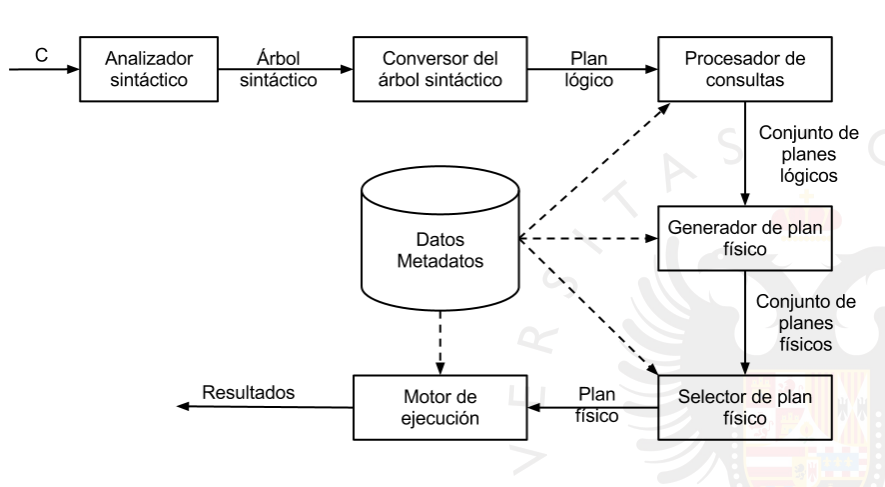
\includegraphics[scale=0.4]{img/1.png}
  \caption{Esquema general de optimización de una consulta}
\end{figure}

\section{Transformación de consultas}

Para transformar la consulta usamos un \textbf{árbol de expresión algebraica} o expresión AR llamado \textbf{plan lógico}. Las hojas de este árbol son las relaciones, los nodos intermedios los operadores y el enlace entre ellos el orden de aplicación.

\begin{example}
El árbol sintáctico $c$ para la siguiente consulta sería:
\begin{lstlisting}[ language=SQL,
                    deletekeywords={IDENTITY},
                    deletekeywords={[2]INT},
                    morekeywords={clustered},
                    framesep=8pt,
                    xleftmargin=40pt,
                    framexleftmargin=40pt,
                    frame=tb,
                    framerule=0pt ]
  SELECT alumno.DNI, alumno.nombre, alumno.calificacion 
  FROM alumno, matricula 
  WHERE alumno.DNI = matricula.DNI 
  AND codigo= "FBD";
\end{lstlisting}
\begin{figure}[H]
  \center
  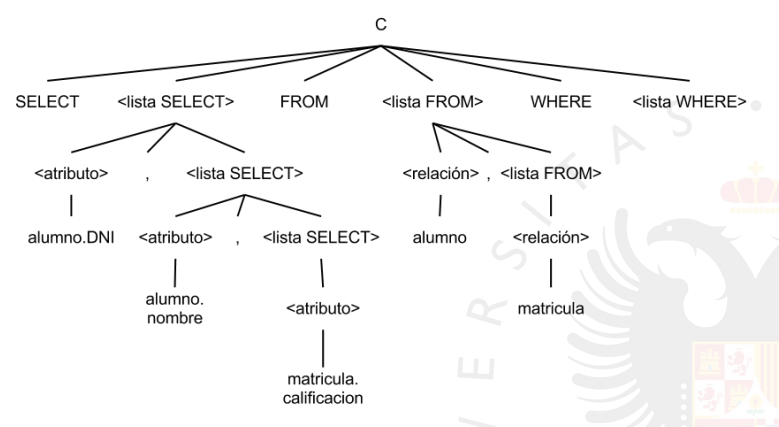
\includegraphics[scale=0.4]{img/2.png}
\end{figure}
Vemos que $<$lista WHERE$>$ no está desarrollado, dos posibles árboles de expresión serían:
\begin{figure}[H]
\centering
\begin{subfigure}{.5\textwidth}
  \centering
  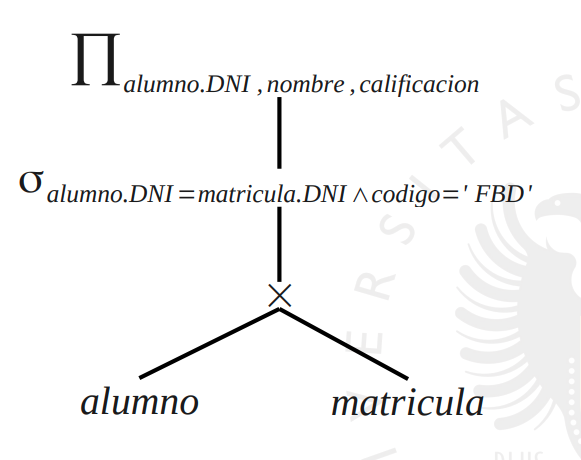
\includegraphics[scale=0.4]{img/3.png}
\end{subfigure}%
\begin{subfigure}{.5\textwidth}
  \centering
  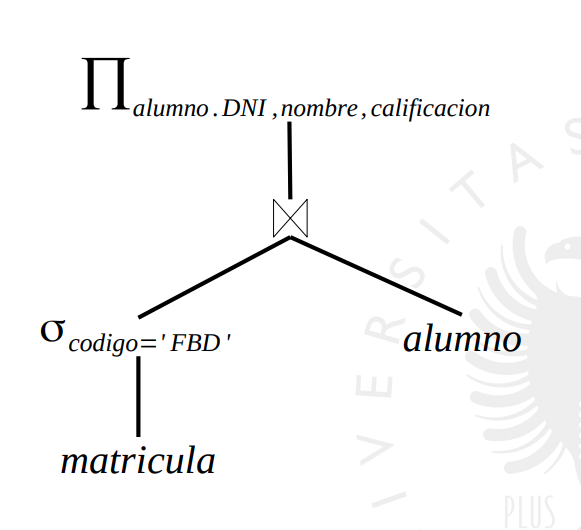
\includegraphics[scale=0.4]{img/4.png}
\end{subfigure}
\end{figure}
\end{example}
Vemos que los dos árboles nos dan un resultado correcto, pero el primero es más costoso de calcular que el segundo. Ahí está la ventaja de estos árboles, mediante una serie de reglas podemos simplicar, eliminar redundancias, etc, para hacer más eficiente una consulta. Algunas de esas reglas son:
\begin{itemize}
\item Conmutatividad de producto, reunión, unión e intersección.
\item Asociatidividad de producto, reunión y unión.
\item Movimiento de selección.
\item Movimiento de proyección.
\item Producto cartesiano.
\end{itemize}
\end{example}

\section{Estrategias para la optimización}
Tenemos varias expresiones equivalentes que difieren en el número de parámetros (tamaño de resultados intermedios, número de tuplas de las relaciones intermedia, etc). El problema es evaluar el coste de cada una, que a su vez también tiene un coste. En general, con $n$ relaciones hay muchas posibilidades:
\[
\frac{(2n-2)!}{(n-1)!}
\]
Un optimizador debe generar un conjunto de planes lo suficientemente amplio para contener el óptimo y lo suficientemente pequeño como para que valga la pena evaluar las posibilidades. Para ello, tenemos varias opciones:
\begin{itemize}
\item Generar un plan según alguna heurística que no es óptimo pero es bueno.
\item Generar todos los planos lógicos posibles, pero sólo funciona para dos relaciones como mucho y crece exponencialmente con la complejidad de la consulta.
\item Una solución mixta: generar un plan seestimargún una heurística y varios planes posibles a partir de él para poder elegir.
\end{itemize}
Cada plan lógico (lo que hay que hacer) genera uno o varios planes físicos (cómo hacerlo), y cada uno incluye:
\begin{itemize}
\item información estadística de datos
\item existencia de índices
\item por cada operador del plan, un algoritmo para aplicarlo
\item los algoritmos de ordenación necesarios
\end{itemize}
Al tener varios planes distintos, necesitamos alguna forma de determinar cuál escoger. Para ello, usamos la estimación de costes. Ejecutar el plan para ver su coste, no es eficiente, obviamente. Además, al principio del plan los datos sobre las relaciones están en el catálogo y conforme avanza la evaluación, dependen de relaciones intermedias y es necesario hacer estimaciones a partir de estadísticas de los datos básicos.

El sistema proporciona algunas estadísticas sobre los datos para ayudarnos a hacer estas estimaciones:

Para una relación ($R$):
\begin{itemize}
\item $N(R)$: número de tuplas de $R$.
\item $L(R)$: longitud en bytes de las tuplas de $R$.
\item $Bfr(R)$: factor de bloqueo de la relación.
\item $B(R)$: número de bloques de la relación $R$.
\end{itemize}
Para un atributo:
\begin{itemize}
\item $V(R,atr):$ número de valores distintos.
\item $nl(R,atr):$ si hay índice sobre el atributo, cuántos niveles tiene un índice multinivel o un B-árbol.
\end{itemize}
Para el sistema:
\begin{itemize}
\item $T(B)$: es el tamaño del bloque en bytes.
\item $C$ es el tamaño de la cabecera del bloque en bytes.
\end{itemize}

\subsection{Tamaño de una proyección}

Dada una relación $R$, la proyección sobre un subconjunto $X$ tendría un tamaño:
\[
L(X)=\sum_{atr_i\in K}size(atr_i)
\]
donde $K$ es el conjunto de atributos del registro. $L$ es la longitud de un registro.
\[
Bfr(X)=\left\lfloor\frac{T(B)-C}{L(X)}\right\rfloor
\]
\[
B(X)=\left\lceil\frac{N(X)}{Bfr(X)}\right\rceil
\]
\begin{example}
Sea la relación $R(a,b,c)$ con $a$ y $b$ enteros ($2B$) y $c$ una cadena de 256 caracteres ($256B$), la cabecera ocupa $16B$ ($C$) y el bloque tiene un tamaño de $T(B)=2048B$. $R$ tiene 1000 registros, es decir $N(R)=1000$.

Calculamos la longitud del registro:
\[
L(R)=2B+2B+256B=260B
\]
Calculamos el factor de bloqueo de esta relación:
\[
Bfr(R)=\left\lfloor\frac{T(B)-C}{L(R)}\right\rfloor=\left\lfloor\frac{2048B-16B}{260B}\right\rfloor=7
\]
Ahora ya podemos calcular el número de bloques de la relación:
\[
B(R)=\left\lceil\frac{N(R)}{Bfr(R)}\right\rceil=\left\lceil\frac{1000}{7}\right\rceil=143
\]
Pero esto es solo para la relación, no para el subconjunto $X$ resultante de la proyección. ¿Cuánto ocupa entonces el resultado de $X=\Pi_{a,b}(R)$? Rehacemos los cálculos pero eliminando de los registros todos los atributos que no aparezcan en la selección, es decir, $N(X)=N(R)=1000$ (porque no eliminamos registros, sino atributos) y $L(X)=2B+2B=4B$.
\[
Bfr(X)=\left\lfloor\frac{T(B)-C}{L(X)}\right\rfloor=\left\lfloor\frac{2048B-16B}{4B}\right\rfloor=508
\]
\[
B(R)=\left\lceil\frac{N(X)}{Bfr(X)}\right\rceil=\left\lceil\frac{1000}{508}\right\rceil=2
\]
\end{example}

\subsection{Tamaño de una selección}

Como el tamaño de la selección depende de cuántos valores cumplan las condiciones de la selección, necesitamos suponer que los datos siguen alguna distribución. La más simple es la uniforme, es decir, la probabilidad de que un atributo tome un valor es un valor constante e igual para todos los valores.

Dada una relación $R$, la selección sobre una condición $c$ tendría un tamaño estimado de
\[
N(X)=\alpha N(R)
\]
donde
\[
\alpha = \left\{
\begin{array}{cl}
\frac{1}{V(R,atr)} & \text{ si } \sigma_{atr=valor}\\
\frac{1}{3} & \text{ si }\sigma_{atr<valor}\\
1 & \text{ si }\sigma_{aatr\neq valor}
\end{array}
\right.
\]
Como una operación de selección no elimina ni añade campos, no afecta a la estructura del registro, luego la longitud y el factor de bloqueo son las mismas tras aplicarla:
\[
L(X)=L(R), \espacio Bfr(X)=Bfr(R)
\]
¿Qué pasa para condiciones compuestas?
\begin{enumerate}
\item Si es una condición AND: aplicamos las selecciones en cascada y multiplicamos los factores de selección.
\item Si es una condición OR: sustituimos por una unión de selecciones y la estimación es:
\[
N(R)\left(1\left(1-\frac{n_1}{N(R)}\right)\left(1-\frac{n_2}{N(R)}\right)\right)
\]
\end{enumerate}

\begin{example}
Base de datos:
\begin{itemize}
\item Alumno (DNI, nombre, fec\_nac, ciudad, direccion, tlfno, beca)
\item Asignatura (codigo, nombre, creditos, caracter, curso)
\item Matricula (codigo, DNI, calificacion)
\end{itemize}
Consulta que queremos optimizar:
\begin{lstlisting}[language=sql]
  SELECT alumno.nombre FROM alumno, matricula 
  WHERE alumno.DNI = matricula.DNI 
  AND beca = "N"
  AND calificacion LIKE "SOBRESALIENTE HONOR%";
\end{lstlisting}
Por simplicidad, usamos la notación:
\[
c_1\equiv \sigma_{beca=N}(Alumnos), \espacio c_2\equiv \sigma_{calificacion=SOBRESALIENTEHONOR}(Matriculas)
\]
Tenemos los siguientes datos de la BD:
\begin{center}
\begin{tabular}{|c|c|c|c|c|}
\hline 
Relación & NTuplas & Bfr & V(Alumnos, Beca) & V(Matrículas, calificacion) \\ 
\hline 
Alumno & 500 & 5 & 2 &   \\ 
\hline 
Matricula & 5000 & 10  &   & 6 \\ 
\hline 
\end{tabular}
\end{center}
Al haber dos valores distintos para Beca, podemos suponer que la mitad tienen beca y la otra mitad no tienen. Luego el número de registros del resultado en $c_1$ sería 250.
\[
N(X)=\frac{1}{V(R,atr)}N(R)=\frac{1}{2}500=250
\]
El factor de bloqueo de $c_1$ es el mismo que el de Alumnos, luego hacen falta 50 bloques para el resultado de $c_1$:
\[
B(R)=\left\lceil\frac{N(X)}{Bfr(X)}\right\rceil=\left\lceil\frac{250}{5}\right\rceil=50
\]
Al haber seis valores distintos para Calificacion, podemos suponer que una sexta parte tienen la calificación buscada. Luego el número de registros del resultado en $c_2$ sería 834:
\[
N(X)=\frac{1}{V(R,atr)}N(R)=\frac{1}{6}5000\approx 250
\]
El factor de bloque de $c_2$ es el mismo que el de Matriculas, luego hacen falta 84 bloques para el resultado de $c_2$:
\[
B(R)=\left\lceil\frac{N(X)}{Bfr(X)}\right\rceil=\left\lceil\frac{834}{10}\right\rceil=84
\]
\end{example}
\subsection{Tamaño de un producto cartesiano}
Este es el más facil de todo, el factor de bloqueo y el número de bloques no cambia, solo el número de registros y la longitud:
Dada una relación $R$, la proyección sobre un subconjunto $X$ tendría un tamaño. Siendo $R$ y $S$ dos relaciones:
\[
N(X)=N(R)N(S)
\]
\[
L(X)=N(R)+N(S)
\]
\[
Bfr(X)=\left\lfloor\frac{T(B)-C}{L(X)}\right\rfloor
\]
\[
B(X)=\left\lceil\frac{N(X)}{Bfr(X)}\right\rceil
\]
\subsection{Tamaño de una reunión natural}
\[
L(X)=L(R)+L(S)-size(b)
\]
donde $b$ es el atributo usado en la reunión natural.

La estimación de $N(X)$ es más compleja y solo se puede hacer si se supone que p ara uno de los atributos de uno de los operandos no se pierde ningún valor al reunir (si había seis valores antes de reunir, hay seis valores después de reunir):
\[
V(R,a)=V(R\;\;JOIN\;\; S,a)
\]
Si la intersección tiene un atributo común, $b$, que toma los mismos malores en ambas tablas:
\[
V(R,b)=V(S,b)
\]
\[
N(X)=\frac{N(R)N(S)}{V(R,b)}=\frac{N(R)N(S)}{V(S,b)}
\]
Si la intersección tiene un atributo en común $b$ y la tabla $S$ hace referencia a la tabla $R$:
\[
V(R,b)\geq V(S,b)
\]
\[
N(X)=\frac{N(R)N(S)}{V(R,b)}
\]
Si la intersección tiene un atributo en común $b$ y la tabla $R$ hace referencia a la tabla $S$:
\[
V(R,b)\leq V(S,b)
\]
\[
N(X)=\frac{N(R)N(S)}{V(S,b)}
\]
Y en general, para que sea más fácil de recordar:
\[
N(X)=\frac{N(R)N(S)}{\max\{V(R,b)V(S,b)\}}
\]
El factor de bloqueo y el número de bloques sigue siendo el mismo:
\[
Bfr(X)=\left\lfloor\frac{T(B)-C}{L(X)}\right\rfloor
\]
\[
B(X)=\left\lceil\frac{N(X)}{Bfr(X)}\right\rceil
\]
\begin{example}
Supongamos la consulta:
\[
R \espacio JOIN \espacio S \espacio JOIN \espacio T
\]
\begin{center}
\begin{tabular}{|c|c|c|}
\hline 
R(a,b) & S(b,c) & T(c,d) \\ 
\hline 
N(R)=5000 & N(S)=3000 & N(T)=1000 \\ 
\hline 
V(R,a)=200 &   &   \\ 
\hline 
V(R,b)=500 & V(S,b)=400 &   \\ 
\hline 
  & V(S,c)=500 & V(T,c)=100 \\ 
\hline 
  &   & V(T,d)=20 \\ 
\hline 
\end{tabular} 
\end{center}
Número de registros:
\begin{figure}[H]
  \center
  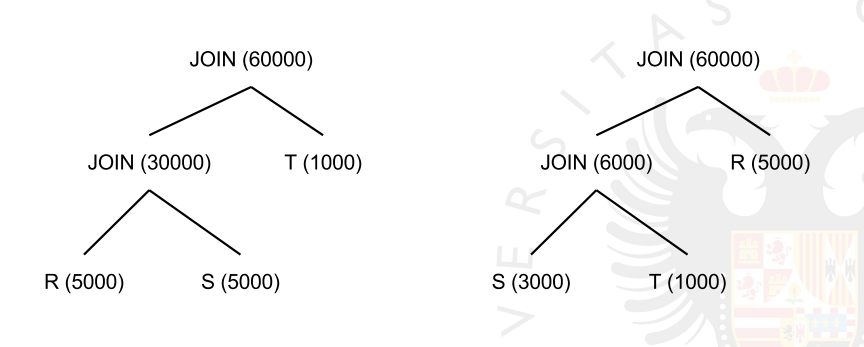
\includegraphics[scale=0.4]{img/7.png}
\end{figure}
Cuidado que hay una errata en el árbol de la izquierda, en el número de registros de $S$, debería ser 3000.
\end{example}
\subsection{¿Cómo trabajan los optimizadores?}
Los SGBD aplican heurísticas de transformación de consultas que, en general, mejoran la eficiencia:
\begin{itemize}
\item Selección lo antes posible.
\item Combinar producto cartesiano y selección en operaciones de reunión.
\item Aplicar la asociatividad para reordenar los nodos hoja de un árbol para realizar las operaciones más restrictivas lo antes posible (lo más a la izquierda y abajo).
\item Proyecciones donde sea posible.
\end{itemize}
